% !TeX program = lualatex
\documentclass[11pt,letterpaper]{article}

%compilar con luatex
\usepackage{fontspec}
\IfFontExistsTF{Avenir Next LT Pro}{
	\setmainfont{Avenir Next LT Pro}
	\setsansfont{Avenir Next LT Pro}
}{
	\setmainfont{TeX Gyre Heros}
	\setsansfont{TeX Gyre Heros}
}
\setmonofont{Noto Sans Mono}[Scale=0.85]

%interlineado de 1.0 
\renewcommand{\baselinestretch}{1.0}

\usepackage[spanish,es-nodecimaldot]{babel}
\usepackage{geometry}
\geometry{top=2.0cm, bottom=2.0cm, left=2.0cm, right=2.0cm}

\usepackage{amsmath,amssymb,amsfonts}
\usepackage{booktabs}
\usepackage{listings}
\usepackage{graphicx}
\usepackage{float}
\usepackage{xcolor}
\usepackage{tikz}
\IfFileExists{microtype.sty}{\usepackage{microtype}}{}
\usepackage{csquotes}

%colores
\definecolor{navyblue}{RGB}{10, 47, 92}
\definecolor{riskred}{RGB}{192, 57, 43}
\definecolor{riskyellow}{RGB}{211, 84, 0}
\definecolor{riskgreen}{RGB}{39, 174, 96}
\definecolor{orcidgreen}{RGB}{166, 206, 57}
\definecolor{codebackground}{HTML}{F4F7FA}
\definecolor{codeframe}{HTML}{D9E2EC}
\definecolor{codecomment}{HTML}{627D98}
\definecolor{codestring}{HTML}{9C4221}

%estilo de bloques de codigo
\lstdefinestyle{bcieR}{
	language=R,
	basicstyle=\ttfamily\small,
	keywordstyle=\color{navyblue}\bfseries,
	commentstyle=\color{codecomment}\itshape,
	stringstyle=\color{codestring},
	backgroundcolor=\color{codebackground},
	frame=single,
	framerule=0.4pt,
	rulecolor=\color{codeframe},
	numbers=left,
	numberstyle=\scriptsize\color{codecomment},
	numbersep=8pt,
	xleftmargin=1em,
	framexleftmargin=1em,
	breaklines=true,
	breakatwhitespace=true,
	showstringspaces=false,
	columns=fullflexible,
	keepspaces=true,
	tabsize=2,
	captionpos=b
}
\lstset{style=bcieR}

%bibliografia
\usepackage[
backend=biber,
style=apa,
citestyle=authoryear
]{biblatex}
\addbibresource{references.bib}

%config de hipervinculos y metadatos
\usepackage{hyperref}
\hypersetup{
	colorlinks=true,
	linkcolor=blue,
	citecolor=blue,
	urlcolor=blue,
	pdftitle={Datathon BCIE - Brecha de Ejecucion en Planes de Adquisiciones},
	pdfauthor={Emerson Lopez}
}

%icono orcid 
\newcommand{\orcidicon}{%
	\raisebox{0.15ex}{%
		\resizebox{2.5mm}{!}{%
			\begin{tikzpicture}[scale=0.0075, baseline=-3pt]
				\fill[orcidgreen] (0,0) circle (256);
				\fill[color=white] (-65,85) rectangle (-115,-115);
				\fill[color=white] (-65,140) circle (30);
				\fill[color=white] (20,140) -- (80,140) .. controls (140,140) and (175,110) .. (175,60) .. controls (175,10) and (140,-20) .. (80,-20) -- (20,-20) -- (20,140);
				\fill[orcidgreen] (55,100) -- (80,100) .. controls (110,100) and (130,85) .. (130,60) .. controls (130,35) and (110,20) .. (80,20) -- (55,20) -- (55,100);
			\end{tikzpicture}%
		}%
	}%
}


\title{%
	\vspace{-1.2cm}
	\Large \bfseries \color{black} Evaluación de la Brecha de Ejecución en los Planes de Adquisiciones del BCIE
}

\author{%
	\textbf{\normalsize Emerson Lopez}\hspace{0.4em}\raisebox{1.2ex}{\href{https://orcid.org/0009-0009-6423-2883}{\orcidicon}} \\
	\footnotesize \href{mailto:emerson.zeledon.ni@gmail.com}{\texttt{emerson.zeledon.ni@gmail.com}} \\
	\footnotesize \href{https://doi.org/10.5281/zenodo.24484873}{DOI}\footnote{Corresponde al código fuente y a la base de datos procesada}\hspace{0.25em}\href{https://doi.org/10.5281/zenodo.24484873}{\texttt{10.5281/zenodo.24484873}} \quad | \quad
	\href{https://github.com/Emerson-nic/Second_Datathon_BCIE}{GitHub} \href{https://github.com/Emerson-nic/Second_Datathon_BCIE}{\texttt{Emerson-nic/Second\_Datathon\_BCIE}}
}

\date{\footnotesize \today}

\begin{document}
	
	\maketitle
	\vspace{-0.4cm}
	
	\section{Análisis Crítico de los Datos y Hallazgos}
	\label{sec:analisis}
	
	Los proyectos de desarrollo necesitan más que financiamiento. También requieren adquisiciones para concretarse en obras, bienes y servicios. La OCDE destaca que la contratación pública es fundamental para la inversión en infraestructura y la prestación de servicios esenciales \parencite{ocde2015procurement}. Por eso importa revisar qué muestran los planes del BCIE. En la muestra principal, el 19.3\% de los procesos figura como pendiente. Estos procesos reúnen el 27.0\% del monto presupuestado, equivalente a USD 1,506,824,159 \parencite{bcie_psd2026}. Esta cifra ayuda a orientar la revisión, pero no demuestra por sí sola que exista un retraso.
	
	\medspace
	
	Este trabajo analiza los planes de adquisiciones vinculados a operaciones financiadas por el \textcite{bcie2025}. La pregunta central es qué parte del presupuesto registrado corresponde a procesos pendientes y qué características se asocian con ese estado.
	
	\medspace
	
	El monto pendiente es la suma de los presupuestos registrados para esos procesos. No representa dinero detenido. Para establecer si hay atrasos harían falta fechas de planificación y de los principales hitos, que no están disponibles en estos registros.
	
	\medspace
	
	Al cruzar los datos\footnote{En este estudio solo se usaron datos del BCIE.} de procesos, planes y operaciones mediante números de préstamo y líneas de crédito, se emparejaron 61 de 71 préstamos identificados (85.9\%). La muestra principal reúne 2,564 procesos de 48 operaciones aprobadas hasta 2022, procesados y consolidados.
	
	La Figura~\ref{fig:estado} compara dos cosas distintas. El panel izquierdo (``monto'') muestra qué porcentaje del presupuesto en dólares corresponde a cada estado. El panel derecho (``procesos'') muestra qué porcentaje del número total de adquisiciones o trámites se encuentra en cada estado.
	
	\medspace
	
	Los estados se agrupan en tres categorías. ``Ejecutado'' incluye los procesos adjudicados, contratados o con contrato terminado. ``Pendiente'' reúne los procesos previstos, en curso, en evaluación, con lista corta o en expresión de interés en curso. ``Fracasado o desierto'' incluye los procesos que constan con esos estados. En número de procesos, 67.5\% está ejecutado, 19.3\% pendiente y 13.2\% fracasado o desierto. En monto presupuestado, lo pendiente representa el 27.0\% del total de la muestra. Aunque estos procesos son menos de una quinta parte del conteo, concentran algo más de una cuarta parte del monto presupuestado, porque cada proceso tiene un monto distinto.
	
	\begin{figure}[H]
		\centering
		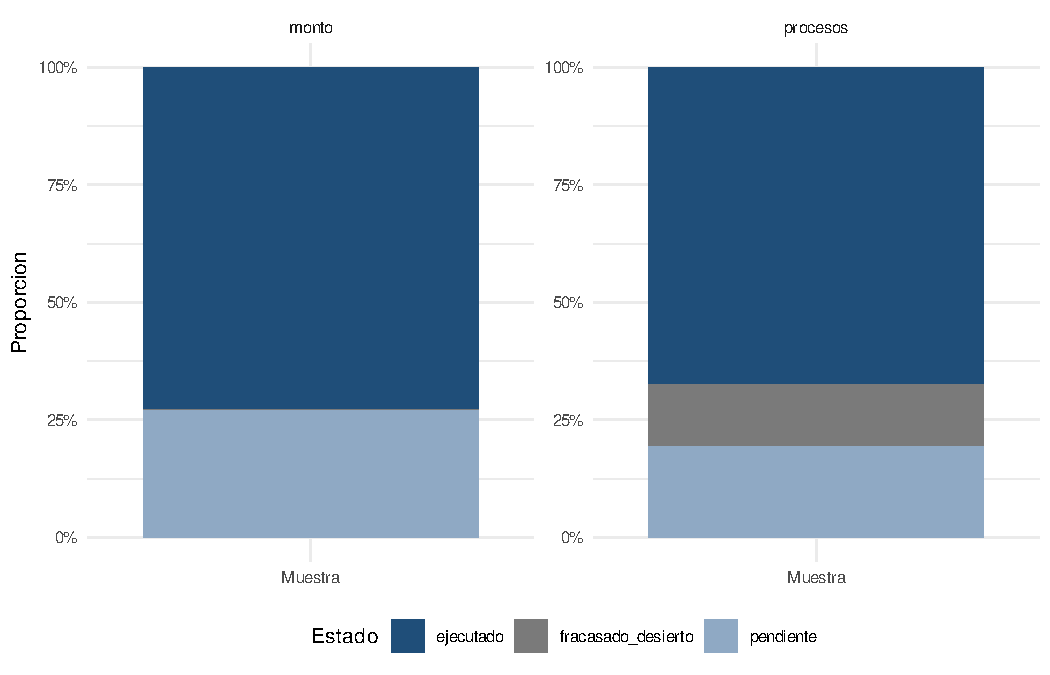
\includegraphics[width = 0.55\textwidth]{../Plots/fig01_estado_conteo_monto.pdf}
		\caption{Distribución porcentual de procesos y presupuesto por estado. Elaboración propia a partir de los datos.}
		\label{fig:estado}
	\end{figure}
	
	
	También destaca una diferencia en los registros. Los procesos fracasados o desiertos son el 13.2\% de los procesos, pero representan solo el 0.24\% del monto presupuestado. En esta muestra, 334 de esos 338 procesos (98.8\%) tienen un monto presupuestado igual a cero. No hay montos faltantes en ese campo. Conviene revisar si esos ceros corresponden a montos realmente iguales a cero o si se usaron para representar información no consignada. Los datos disponibles no permiten determinar la causa. Esta revisión puede ayudar a mejorar la calidad de los datos abiertos del Banco.
	
	\section{Metodología y Proceso de Análisis}
	\label{sec:metodologia}
	
	Todo el procesamiento de datos, el análisis descriptivo y el ajuste del modelo se hicieron en R con los paquetes \texttt{stats} \parencite{stats_pkg} y \texttt{lmtest} \parencite{zeileis2002lmtest}, a partir del código y los datos procesados por \textcite{zeledon2026bcie}. La base reúne 2,564 procesos de 48 operaciones aprobadas hasta 2022, vistos una sola vez en el corte de 2026, es decir, es un corte transversal~\footnote{Cada proceso se observa una sola vez en el corte de datos disponible (operaciones aprobadas hasta 2022 observadas en 2026), sin seguimiento a lo largo del tiempo.}. Para ver qué características se asocian con estar pendiente usamos un modelo logit binario~\footnote{Una variable binaria o dicotómica solo toma dos valores posibles (aquí $1$ o $0$), como ``sí/no'' o ``pendiente/no pendiente''.} \parencite{cox1970analysis}. Como antecedente cercano, \textcite{he2023procurement} estiman con un modelo logit la probabilidad de retraso en contratos públicos del Reino Unido y complementan el análisis con modelos de duración, aunque, su estudio no es idéntico a este. Se estima la probabilidad de que un proceso figure como pendiente, porque los datos del PSD no incluyen fechas suficientes para medir retrasos. La variable dependiente $Y_{ij}$ vale $1$ si el proceso está pendiente y $0$ en los demás casos.
	
	\medspace
	
	El modelo incluye la categoría del proceso, su presupuesto, su peso dentro del plan (\textit{share}), el monto aprobado de la operación, la relación entre el plan y el monto aprobado, el número de procesos y la antigüedad (edad) de la operación. El monto del proceso y el monto aprobado se transformaron como $\log(1+x)$, lo que reduce la influencia de las diferencias grandes de escala. En R, el modelo base se estima de la siguiente manera.
	
	\begin{center}
		\begin{minipage}{0.88\textwidth}
			\begin{lstlisting}[language = R, basicstyle = \ttfamily\small, breaklines = true, frame = single]
				modelo <- stats::glm(
				pendiente ~ categoria_proceso + log_monto_proceso + share_plan +
				log_monto_aprobado + plan_sobre_aprobado + n_procesos + edad,
				data = datos,
				family = stats::binomial
				)
			\end{lstlisting}
		\end{minipage}
	\end{center}
	
	Como varios procesos pertenecen a una misma operación, agrupamos los errores estándar por número de préstamo con la función \texttt{vcovCL} del paquete \texttt{sandwich} y la función \texttt{coeftest} del paquete \texttt{lmtest} \parencite{zeileis2020sandwich, zeileis2002lmtest}. El modelo no incluye país ni sector, y los resultados muestran asociaciones estadísticas. En la ecuación, $Y_{ij}$ indica si el proceso $i$ de la operación $j$ está pendiente y $\mathbf{X}_{ij}$ reúne sus variables.
	
	\begin{equation}
		P(Y_{ij} = 1 \mid \mathbf{X}_{ij}) = \Lambda(\mathbf{X}_{ij}\boldsymbol{\beta}) = \frac{1}{1 + e^{-\mathbf{X}_{ij}\boldsymbol{\beta}}}
	\end{equation}
	
	\noindent En pocas palabras, esta fórmula convierte las características del proceso en una probabilidad estimada de estar pendiente. Sirve para ordenar dónde conviene revisar primero, pero no predice fechas de ejecución ni asegura lo que pasará con un proceso en particular.
	
	\section{Visualizaciones y Resultados}
	\label{sec:resultados}
	
	En los 2,564 procesos analizados, los resultados del modelo logit con errores agrupados por operación muestran que solo tres variables tienen una asociación estadísticamente significativa con estar pendiente (sus intervalos de confianza del 95\% no incluyen el $1.00$), tal como se muestra en la Figura~\ref{fig:odds-ratios}, el monto del proceso en escala logarítmica, su participación en el plan y la relación entre el plan y el monto aprobado. Las demás variables, las categorías de adquisición frente a \textit{Bienes}, el monto aprobado de la operación, el número de procesos y la antigüedad, no muestran una diferencia clara en este modelo.
	
	\begin{figure}[H]
		\centering
		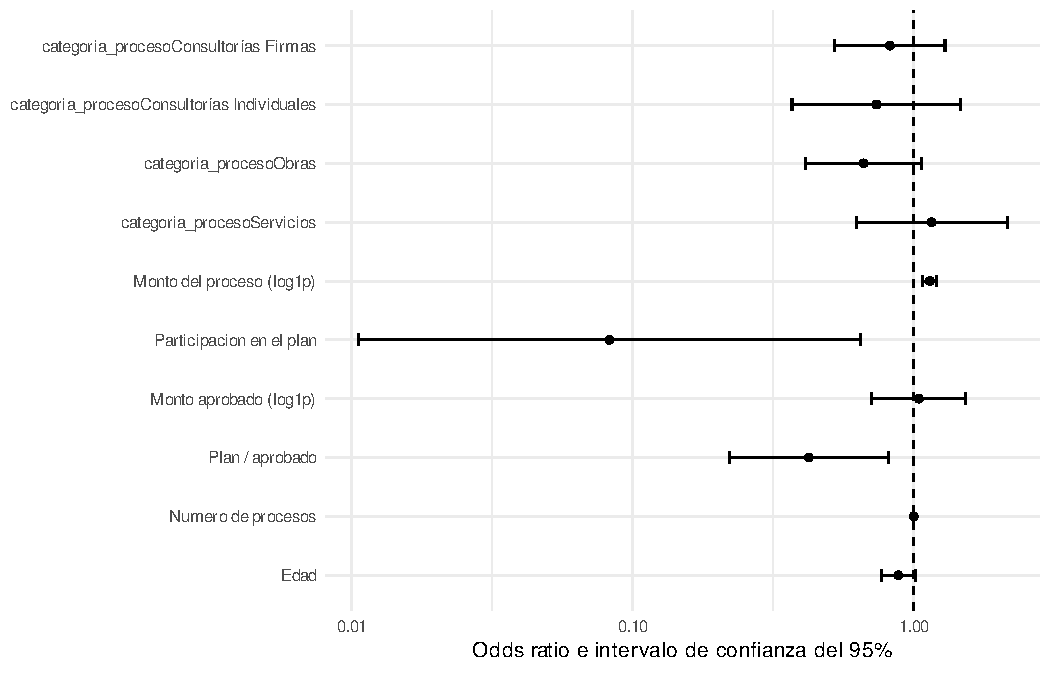
\includegraphics[width = 0.55\textwidth]{../Plots/fig06_odds_ratios.pdf}
		\caption{Razones de momios e intervalos de confianza del 95\%. Los errores estándar se agrupan por operación y \textit{Bienes} es la categoría de referencia. Elaboración propia.}
		\label{fig:odds-ratios}
	\end{figure}
	
	Para interpretar las 3 asociaciones se utiliza odds ratio (OR) o razón de momios, compara los momios de que un proceso figure pendiente entre distintos valores de una variable, manteniendo constantes las demás.
	
	\begin{itemize}
		\item \textbf{Monto del proceso ($\log(1 + \text{monto})$):} el OR es $1.14$ por cada unidad en la escala logarítmica (IC 95\% entre $1.08$ y $1.21$). En términos prácticos, subir de un proceso de USD $1$ millón a uno de USD $2$ millones se asocia con momios cerca de $9.5\%$ más altos de estar pendiente (IC 95\% entre $5.2\%$ y $13.9\%$), manteniendo lo demás constante.
		\item \textbf{Participación en el plan:} al pasar de $10\%$ a $20\%$ de participación, el OR es $0.78$ (IC 95\% entre $0.63$ y $0.96$). Es decir, se asocia con momios $22\%$ menores de figurar pendiente (con un rango compatible de entre $4\%$ y $37\%$ menos). Si se mira el cambio en una unidad completa ($100$ puntos porcentuales), el OR es $0.08$ (IC 95\% entre $0.01$ y $0.64$).
		\item \textbf{Relación plan / monto aprobado:} si esta proporción sube, por ejemplo, de $0.5$ a $1.5$, el OR es $0.42$ (IC 95\% entre $0.22$ y $0.81$). Esto se asocia con momios $58\%$ menores de estar pendiente (con un rango compatible de entre $19\%$ y $78\%$ menos).
	\end{itemize}
	
	
	El modelo también ayuda a ordenar y priorizar qué operaciones revisar primero. En el panel A de la Figura~\ref{fig:clasificacion-top10}, cada punto representa una operación, donde el eje horizontal muestra la proporción pendiente esperada, el eje vertical el monto pendiente esperado en escala logarítmica para apreciar mejor las diferencias de tamaño y el tamaño del punto la antigüedad de la operación. Los colores dividen las operaciones en tres terciles según su proporción pendiente esperada, funcionando como un semáforo visual para ubicar rápido los grupos de menor, media y mayor participación pendiente, mientras las líneas punteadas en 30\% y 60\% actúan como referencia.
	
	\medspace
	
	En el panel B, el top 10 ordena las operaciones de mayor a menor según su monto pendiente esperado, calculado al sumar el presupuesto de cada proceso multiplicado por su probabilidad estimada de estar pendiente. Muchas de estas operaciones con mayor monto pendiente esperado coinciden con el tercil superior de mayor propensión o proporción pendiente, aunque una operación con menor porcentaje puede subir en el ranking si su presupuesto total es grande. El rojo en las barras resalta las diez operaciones con mayor monto pendiente esperado para facilitar su revisión.
	
	\begin{figure}[H]
		\centering
		\begin{minipage}[t]{0.48\textwidth}
			\centering
			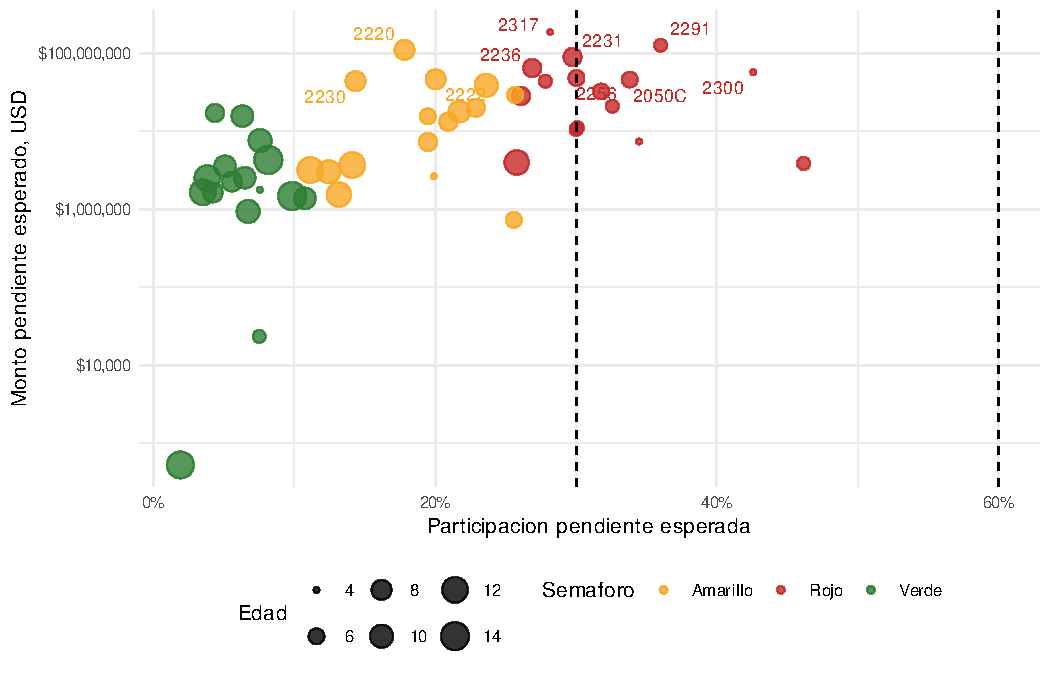
\includegraphics[width = \linewidth]{../Plots/fig03_dispersion_share_monto.pdf}
			\par\small Panel A. Proporción y monto pendiente esperado por operación.
		\end{minipage}\hfill
		\begin{minipage}[t]{0.48\textwidth}
			\centering
			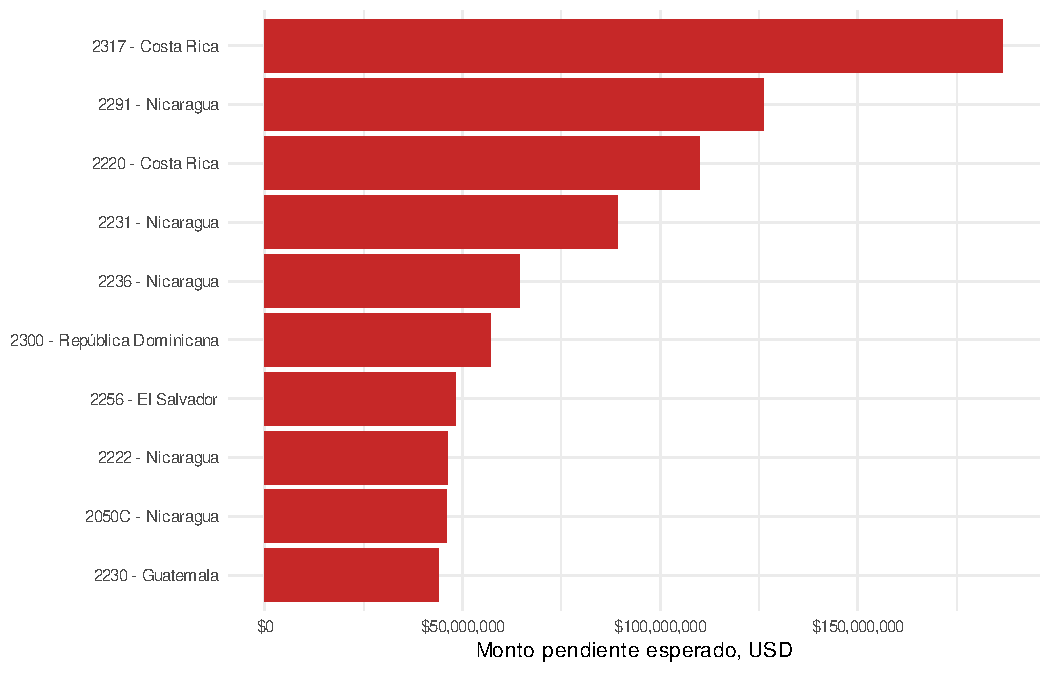
\includegraphics[width = \linewidth]{../Plots/fig04_top10.pdf}
			\par\small Panel B. Diez operaciones con mayor monto pendiente esperado.
		\end{minipage}
		\caption{Clasificación y priorización de operaciones. Elaboración propia.}
		\label{fig:clasificacion-top10}
	\end{figure}
	
	\section{Propuesta Concreta de Mejora}
	\label{sec:propuesta}
	
	A partir de los resultados del modelo y del análisis de la cartera, conviene usar la clasificación por terciles y el listado de las diez operaciones con mayor monto pendiente esperado como una agenda práctica para las revisiones periódicas. Como parte de esta propuesta, se desarrolló un dashboard interactivo en \href{https://connect.posit.cloud/em3r/content/01a20a50-e45d-b6b9-9e3c-9c72aaae51a9}{Posit Connect} que permite a los equipos del Banco explorar las operaciones, aplicar filtros por país o categoría y visualizar el semáforo de riesgo en tiempo real. El equipo encargado puede revisar primero las operaciones que aparecen en el tercil superior o en el top 10 para contrastar el estado con el expediente, comprobar si el plan y el monto siguen vigentes y ver si hace falta apoyo o actualización. Esta clasificación ordena la atención, pero no reemplaza el criterio del equipo ni debe leerse como una evaluación de desempeño.
	
	\medspace
	
	Para armar esa guía, las probabilidades estimadas de los procesos se ponderan por su monto presupuestado y se suman por operación. La regla del semáforo marca en rojo una proporción pendiente estimada de al menos 60\%, o de al menos 40\% en operaciones con seis años o más. Marca en amarillo una proporción de al menos 30\% que no llega al umbral rojo, y en verde una proporción menor a 30\%. En esta muestra ninguna operación queda en rojo bajo esa regla absoluta. El listado de diez operaciones, en cambio, ordena según el monto pendiente esperado y combina tanto la probabilidad estimada como el tamaño del presupuesto.
	
	\medspace
	
	Una mejora de fondo sería publicar fechas de planificación, convocatoria, evaluación, adjudicación y contrato, además de mantener al día los estados y revisar la integridad de los montos. Con esas fechas sería posible distinguir entre una actividad que sigue su curso previsto y una demora real. Mientras no existan esas fechas en los registros públicos, el estado pendiente no debe tomarse como sinónimo de retraso. Asimismo, la diferencia entre el porcentaje de procesos fracasados o desiertos y su peso en el monto registrado ofrece una buena oportunidad para revisar y mejorar la calidad de los datos abiertos del Banco, no para buscar culpables.
	
	\section*{Referencias}
	\label{sec:referencias}
	
	\printbibliography[heading=none]
	
	\newpage
	\appendix
	\section{Anexo}
	\label{sec:anexo}
	
	Todo el pipeline de datos, los scripts de estimación econométrica en R y la aplicación interactiva se desarrollaron bajo principios de ciencia abierta y transparencia metodológica. El código fuente de este proyecto se encuentra publicado bajo la licencia de código abierto MIT, lo que permite su uso, modificación y adaptación libre por parte del equipo técnico del BCIE o de cualquier entidad interesada en implementar esta herramienta de priorización.
	
	\medspace
	
	Tanto la base de datos procesada como el código completo de análisis y visualización se encuentran preservados en Zenodo con un \href{https://doi.org/10.5281/zenodo.24484873}{DOI permanente} y alojados en el repositorio público de \href{https://github.com/Emerson-nic/Second_Datathon_BCIE}{GitHub}. Por su naturaleza modular y su licencia permisiva, se recomienda la adopción, reutilización y mejoramiento de este código como metodológico para base para futuras integraciones de analítica preventiva dentro de los sistemas institucionales de datos abiertos.
	
	\medspace
	
	
	
	
\end{document}	